\chapter{Deep Leaning}

% Fazer um resumo

Um dos clássicos problemas na área
de classificação de imagens era o
reconhecimento de dígitos
escritos à mão. 
A dificuldade nesse tipo de problema
vinha pela grande variação de forma
e posição dos números, tornando 
os modelos muito complexos e pouco
precisos. O desenvolvimento
recente na área de Machine Learning
permitiu a criação de modelos
simples capazes de aprender com
os dados e fazer generalizações
precisas, em alguns casos
superando a percepção humana.

Neste capítulo serão apresentadas
técnicas que usam Redes Neurais,
como elas foram desenvolvendo
ao longo dos anos, e como podemos
aplicá-las na Síntese de Textura.


%\cite{Li2021}

\section{Aprendizado de Representação}
%19h


% Hierarquia de representações
No processo de análise de imagens,
precisamos criar representações
que melhor explicam seu conteúdo.
Essas representações podem ser organizadas
hierarquicamente, onde
a primeira identifica
arestas, a segunda indica cantos, etc.
Ao descer no nível das representações
queremos ter uma melhor informação
semântica da imagem.


Para um problema de classificação de imagens,
é preciso saber quais informações são 
úteis para obter uma melhor 
representação de seu conteúdo. 
Uma representação boa esconde informações
redundantes e realça fatores que 
melhor explicam a imagem.
Bengio, Courville e Vincent
\cite{Bengio2014} falam do importante
papel que a aprendizagem
de representações tem em Machine Learning.
Um algoritmo que aprendesse tais representações
eliminaria o trabalho de desenvolvê-las,
o que tornaria mais rápido a criação de aplicações.


\section{Redes neurais}
%20h

% Definir o que é uma rede neural


Redes Neurais são um tipo 
de modelo de Machine Learning inspirado
em redes de neurônios naturais e como
eles se comunicam. Elas podem ser
representadas por um grafo, onde
cada nó representa um valor e cada aresta
representa uma dependência. Essas
redes podem ter vários formatos
dependendo do tipo de aplicação.

Um exemplo comum de Rede Neural é o Multi Layer
Perceptron. Nesse modelo, a rede é dividida
em camadas de diferentes tamanhos, e o dado
flui da camada de entrada até a saída,
que pode representar uma classificação
da entrada ou uma função geral.

% Imagem MLP

\begin{figure}[!ht]
	\centering
	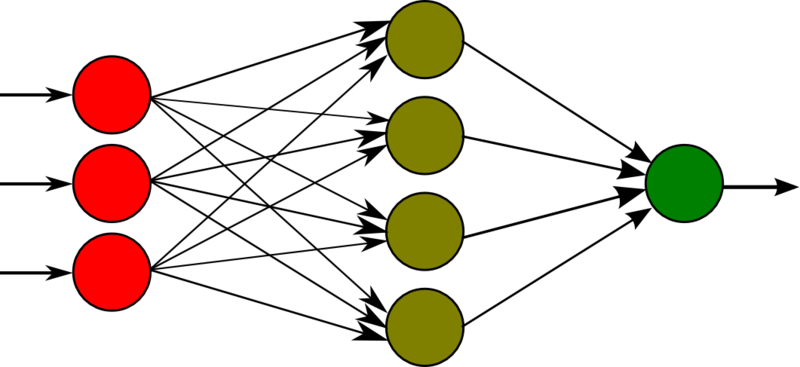
\includegraphics[width=\linewidth*2/3]{files/assets/deeplearning/mlp.png}
	\caption{Rede Multi Layer Perceptron. Cada camada da
	rede atua como uma representação do dado de entrada, que
	é usada para calcular a próxima camada.}
	\label{img:preview}
\end{figure}


Cada camada da rede tem como parâmetros os offsets 
$\mathbf{b}_m$ e uma matriz de pesos $\mathbf{W}_{m\times n}$.
Assim, a transformação da entrada $\mathbf{x}_n$ na saída
$\mathbf{y}_m$ pode ser representada com a seguinte operação:
\begin{equation}
	\mathbf{y} = 
	\varphi\left( \mathbf{W}\mathbf{x} + \mathbf{b} \right),
\end{equation}
onde $\varphi$ é uma função não linear, comummente chamada
de ``função de ativação''. A função não linear
mais comummente usada é a ReLU, que trunca valores
negativos no $0$.

\begin{figure}[!ht]
	\centering
	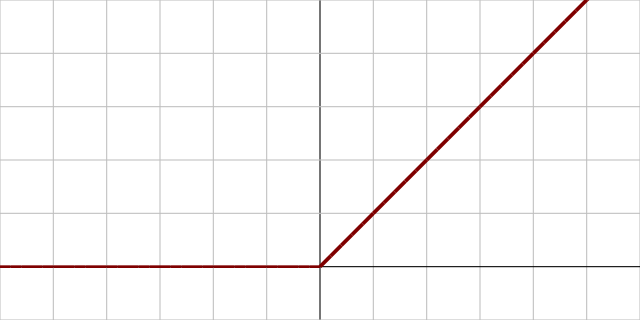
\includegraphics[width=\linewidth*2/3]{files/assets/deeplearning/relu.png}
	\caption{Função ReLU. O seu bico não diferenciável
	facilita a distorcer o espaço de entrada.}
	\label{img:preview}
\end{figure}

%Os parâmetros são tais que minimizam o erro 
%da saída. Essa minimização pode ser feita
%calculando o gradiente 
%\begin{equation}
%	\mathbf{y'} = 
%	\mathbf{W}\varphi'\left( \mathbf{W}\mathbf{x} + \mathbf{b} \right),
%\end{equation}

Os parâmetros são calculados minimizando
uma função de erro na saída. Essa minimização
é feita usando o gradiente dos parâmetros
em relação à função de perda. Como a derivada
de todas as funções aplicadas é conhecida,
o gradiente pode ser calculado computacionalmente
utilizando ``backpropagation''.

%A ideia é ter um modelo
%simples porém bem flexível
%e capaz adaptar ao problema.

% Aproximado universal para qualquer função
% Capacidade de extrapolação

% Dividir qualquer variedade

Esse modelo é útil por envolver operações
bem simples e rápidas de serem calculadas
computacionalmente. Cada camada distorce
o espaço de entrada para torná-lo linearmente
separável no final. Pela sua flexibilidade,
o modelo geralmente é chamado de aproximador 
universal de qualquer função, pois
é capacidade de aprender funções complexas
a partir de amostras.


% Falar do MNIST
%...

\section{Redes convolucionais}
%21h

% Aproveitam a informação espacial
% da imagem

% Reduz a quantidade de parâmetros
% Invariante por translação

O Multi Layer Perceptron (MLP),
quando aplicado diretamente
nos pixels de uma imagem aparecem
dois problemas consideráveis:
a quantidade de parâmetros cresce muito,
e informações espaciais da imagem
são perdidas. Geralmente um objeto
que queremos identificar pode aparecer
em diferentes posições da imagem,
e ao transformá-la em um vetor,
perdemos essa invariância por translação.
Com base nisso se tornou necessário
desenvolver uma rede que aproveite
a informação espacial da imagem
e que tenha poucos parâmetros.

% Sobre convolução
%A operação de convolução

A convolução é um filtro linear 
muito utilizado em processamento
de imagens. Para transformar
a imagem ele recebe uma matriz
chamada kernel, e faz a convolução
somando a vizinhança de cada ponto
com os pesos definidos pelo kernel.
Dependendo da matriz escolhida,
vários filtros podem ser gerados,
como detector de arestas, suavizador,
etc.

\begin{figure}[!ht]
	\centering
	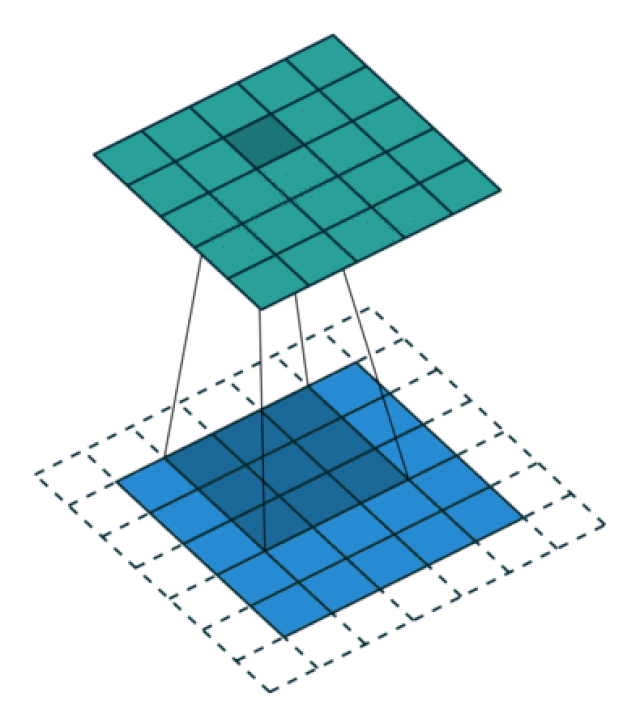
\includegraphics[height=200pt]{files/assets/deeplearning/conv.png}
	\caption{Exemplo de como a convolução opera em uma imagem.
	Em azul a origem e em verde o destino. O kernel nesse caso
	é uma matriz $3\times 3$. A imagem precisa ser extrapolada
	para as vizinhanças das bordas, geralmente é preenchida
	com 0.}
	\label{img:preview}
\end{figure}


% Sobre CNN (pooling, ReLU)

Uma rede neural convolucional é formada
por um conjunto de convoluções que
geram representações da entrada, 
tendo o kernel como parâmetro a ser aprendido.
A rede empilha essas convoluções seguidas
de aplicações de funções ReLU para tirar
a linearidade, e camadas de Pooling,
que diminuem o tamanho da imagem
juntando pixels vizinhos através de
operações como a média ou o máximo.


Uma imagem na entrada da rede tem 
dimensão $W\times H \times 3$,
onde a última representa os três
canais de cores.
As convoluções operam nos canais
de cores e podem gerar novos canais,
geralmente chamados de ``features'',
cada uma representando alguma informação
da imagem.
% !!! Falar do aumento de features

% Revolução na classificação

Esse tipo de rede gerou uma revolução
no ramo de classificação de imagens.
A classificação era feita passando
por algumas camadas de Pooling e
ligando a saída em uma rede Multi
Layer Perceptron.

Uma exemplo de arquitetura que obteve
sucesso em classificação de imagens
foi a rede VGG-19. Essa rede 
tem camadas de convolução e ReLU,
e a cada pooling dobra o número
de features, indicando que quanto
mais abaixo a informação está na rede,
mais representações ela pode ter.

\begin{figure}[!ht]
	\centering
	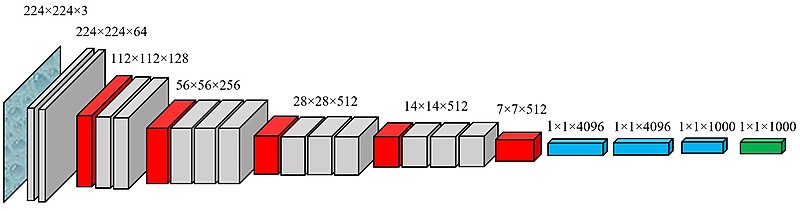
\includegraphics[width=\linewidth*5/6]{files/assets/deeplearning/vgg19.png}
	\caption{Arquitetura da rede VGG-19. Cada bloco cinza representa
	uma convolução e um ReLU, os blocos vermelhos representam 
	Pooling, os blocos azuis são camadas da rede MLP e em verde é a
	saída da classificação (ela é treinada para diferencias $1000$
	classes).}
	\label{img:preview}
\end{figure}

%\section{Features}

% Mostrar o feature inversion
% e o deep dream 



\section{Síntese de textura com Redes Convolucionais}
%22h

As redes convolucionais
treinadas para classificação de imagem (em particular
a rede VGG-19) fazem uma série de operações em
pirâmide para extrair informação úteis da imagem que
se quer classificar. A riqueza semântica de cada
uma dessas informações vai depender do nível da camada,
com as primeiras camadas salientando detalhes
mais primitivos, como arestas e cantos, e as últimas
camadas salientando objetos complexos como rostos
e animais.

% Deep dream?

Para a criação do método de síntese de textura
utilizando essas redes, a equipe de Gatys percebeu que 
mantendo as relações entre as camadas,
a textura pode ser randomizada sem que 
a informação perceptual da imagem se perca.
Para isso eles utilizaram a matriz de Gram gerada por cada
uma dessas camadas. A matriz tem tamanho $N_l \times N_l$,
onde $N_l$ é o número de features da camada $l$ da rede.
A saída de cada camada convolucional tem dimensão
$W_l\times H_l \times N_l$; para calcular a matriz de Gram
definimos $F_l$ como sendo uma planificação da 
saída da camada, ou seja, $F_l$ tem dimensão $N_l \times (W_l H_l)$.
Assim, $G_l = F_lF_l^T$. Essa matriz é útil pois ela não 
depende da resolução da imagem que entrou na rede,
assim pode ser usada para gerar imagens em
qualquer resolução.

A geração da textura é feita através de algoritmo
de otimização baseado em gradiente. Para isso
comparamos as matrizes de gram da amostra e da
imagem sendo gerada para calcular o gradiente
com respeito a perda quadrática. Em seguida
a imagem é atualizada para diminuir essa perda,
forçando-a a ter as mesmas auto-correlações entre
as features.

\begin{figure}[!ht]
	\centering
	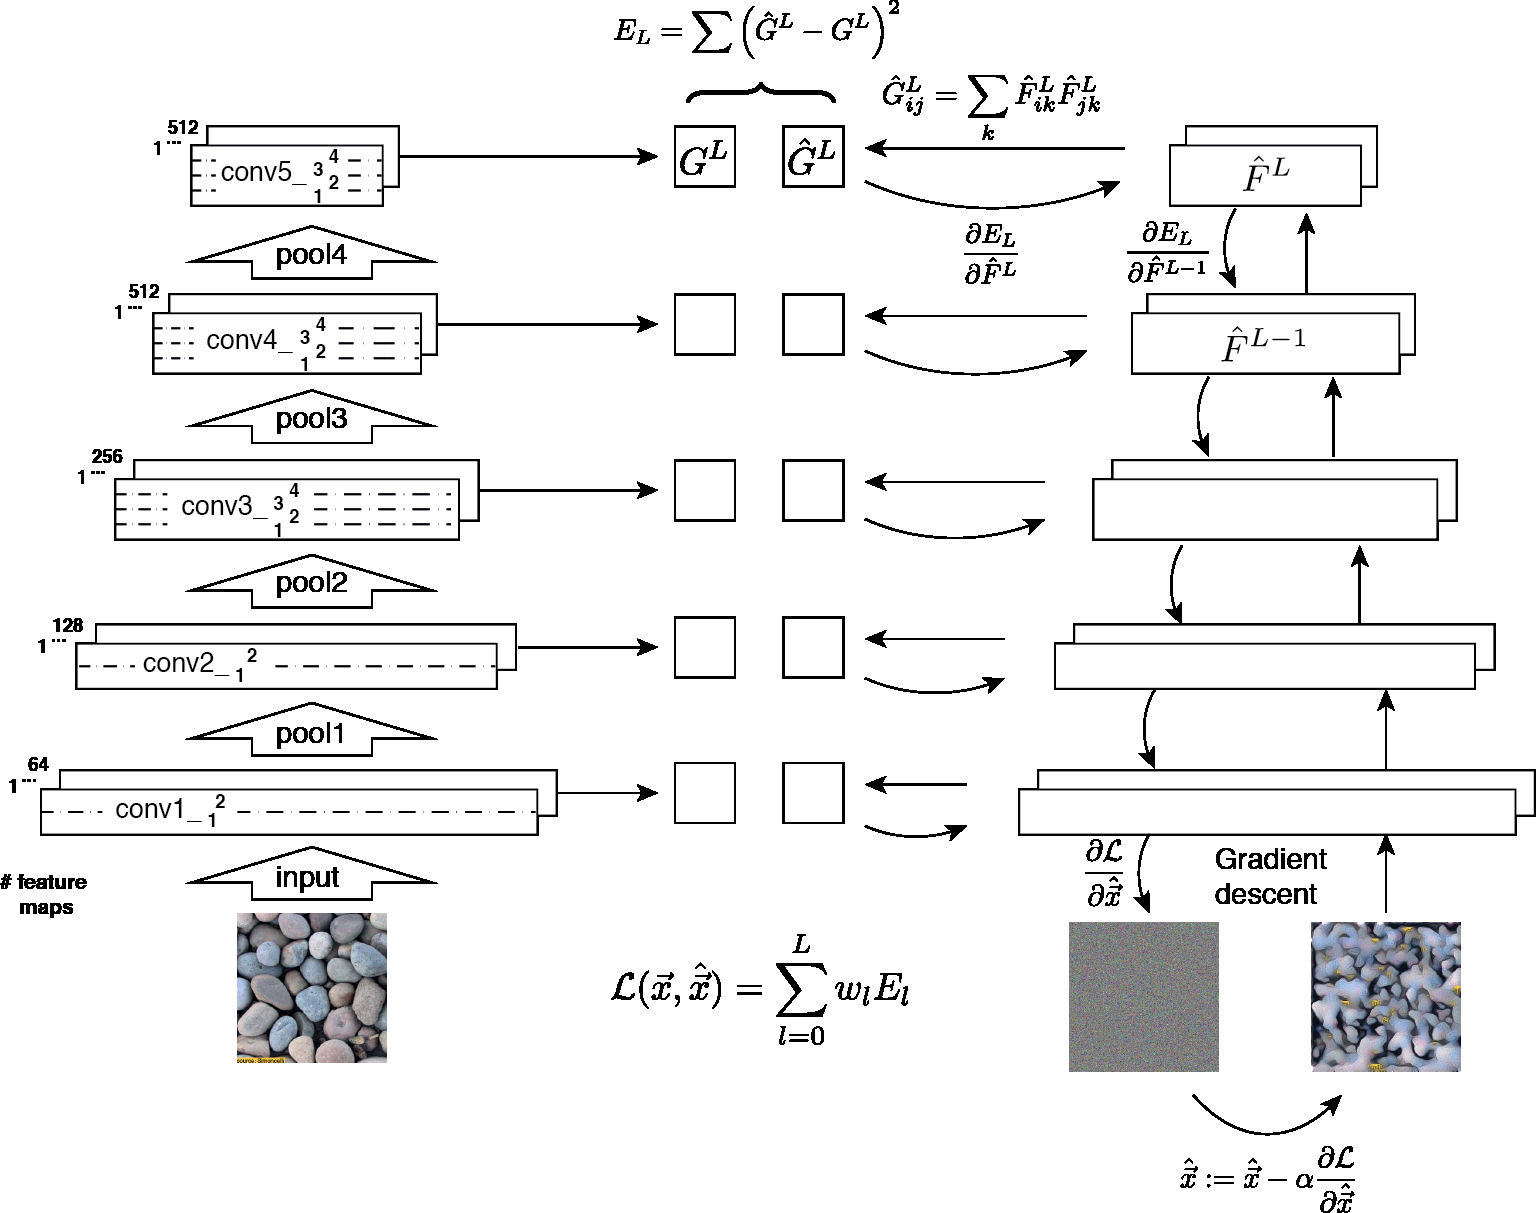
\includegraphics[width=\linewidth*2/3]{files/assets/articles/gatys2.png}
	\caption{Esquema do método de Gatys. Para a otimização
		é utilizado o algoritmo L-BFGS, 
		que avalia o resultado da função
		várias vezes antes de fazer o passo,
		e é mais eficiente em problemas de grande quantidade
		de parâmetros.}
	\label{img:preview}
\end{figure}


 

% Falar do L-BFGS 
% (avalia o resultado da função várias vezes
% antes de fazer o passo, é mais eficiente
% em problemas com grande quantidade de parâmetros)

% Falar do padding e do avgpool


% Mostrar os resultados do Gatys

%\section{} %MSLG+Gatys

\iftrue
\chapter{Variações}

O trabalho de síntese de textura
não fica limitado apenas a re-amostrar
a imagem de entrada. Ao longo
dos anos foram aparecendo trabalhos
que aproveitavam os algoritmos
desenvolvidos até então para
criar aplicações como ``inpainting''
e ``renderizações não foto-realísticas''.


% Falar de aplicações diferendes de síntese de
% textura

Neste capítulo será falado de duas
variações bem interessantes de síntese
de textura, que nos permitem ter mais
controle do conteúdo no resultado.


\section{Analogias de Texturas}

O método de analogias de texturas
foi proposto no trabalho de 
Hertzmann, Jacobs, Oliver, Curless
e Salesin \cite{Hertzmann2001}.
O algoritmo consiste em fazer analogias
de imagens, ou seja, ele
recebia três imagens, $A$, $A'$ e $B$,
e tentava gerar $B'$ de modo que
$A'$ esteja para $A$ assim como
$B'$ estará para $B$.


\begin{figure}[!ht]
	\centering
	
	\begin{tabular}{ccccccc}
	\raisebox{-.5\height}{
	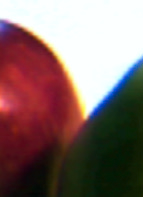
\includegraphics[height=80pt]{files/assets/articles/hz5.png}}
	& $:$ &
	\raisebox{-.5\height}{
	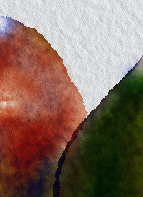
\includegraphics[height=80pt]{files/assets/articles/hz6.png}}
	& $::$ &
	\raisebox{-.5\height}{
	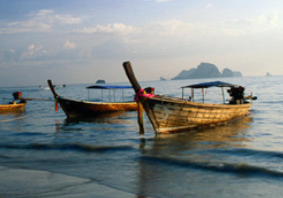
\includegraphics[height=80pt]{files/assets/articles/hz7.png}}
	& $:$ &
	\raisebox{-.5\height}{
	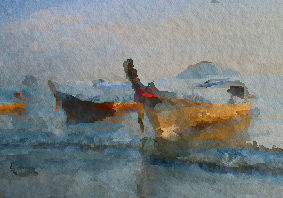
\includegraphics[height=80pt]{files/assets/articles/hz8.png}}\\
	$A$&&$A'$&&$B$&&$B'$
	\end{tabular}

	\caption{Exemplo de analogia de imagens. As relações
	entre $A'$ e $A$ devem ser aplicadas em $B$ para gerar $B'$.}
	\label{img:preview}
\end{figure}

O algorítimo faz a síntese utilizando
a representação multi-escala das imagens,
gerando da camada mais grosseira até a camada
mais fina. A geração é feita pixel por pixel,
e leva em conta a sua vizinhança em $B$ e 
vizinhança de seu correspondente em $A$.
%CITAR IMAGEM


\begin{figure}[!ht]
	\centering
	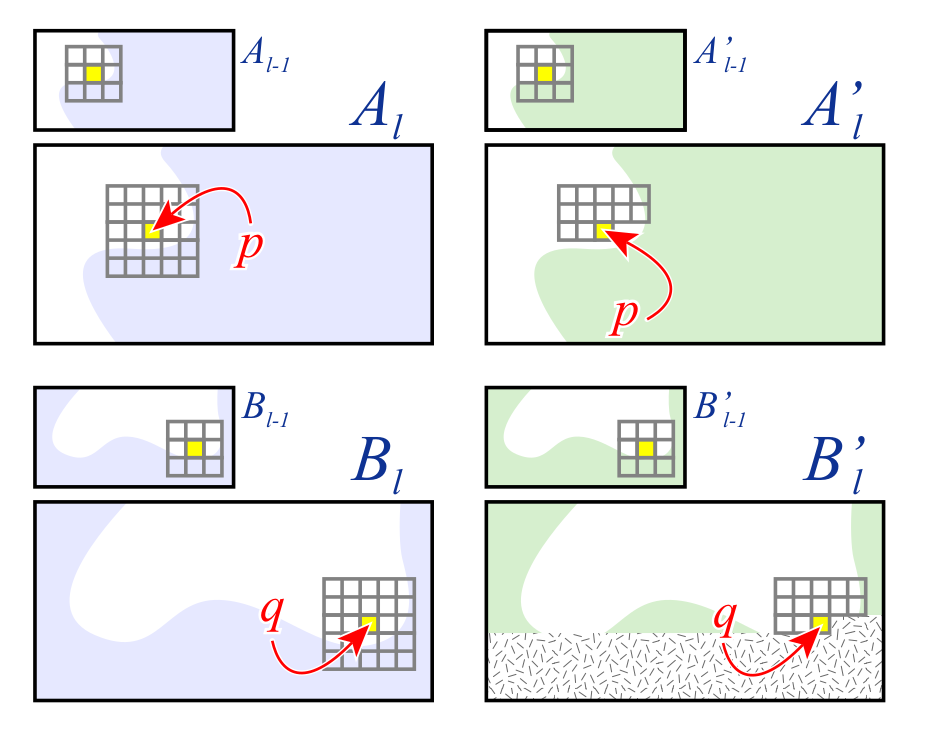
\includegraphics[width=\linewidth*2/3]{files/assets/articles/heartzmann2.png}
	\caption{Para gerar o pixel $q$ da camada $l$, o algoritmo
	usa a vizinhança correspondente em $B_l$, $B'_{l-1}$ e $B_{l-1}$.
	Ele busca o melhor correspondente nas imagens $A$.}
	\label{img:preview}
\end{figure}

\begin{figure}[!ht]
	\centering
	
	\begin{tabular}{ccccccc}
	\raisebox{-.5\height}{
	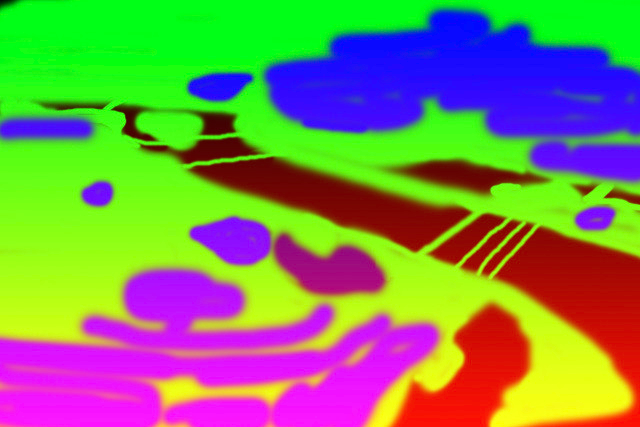
\includegraphics[height=55pt]{files/assets/articles/hz1.png}}
	& $:$ &
	\raisebox{-.5\height}{
	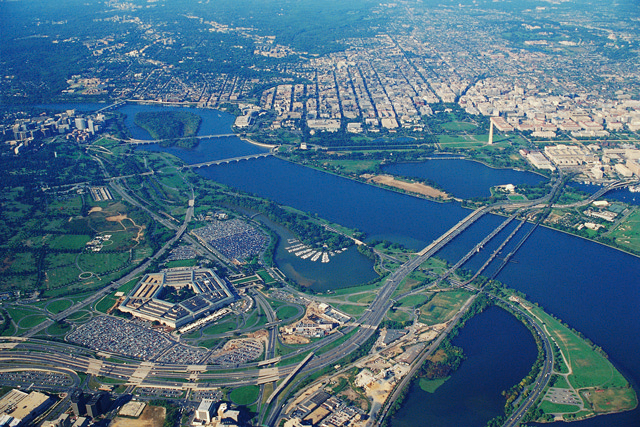
\includegraphics[height=55pt]{files/assets/articles/hz2.png}}
	& $::$ &
	\raisebox{-.5\height}{
	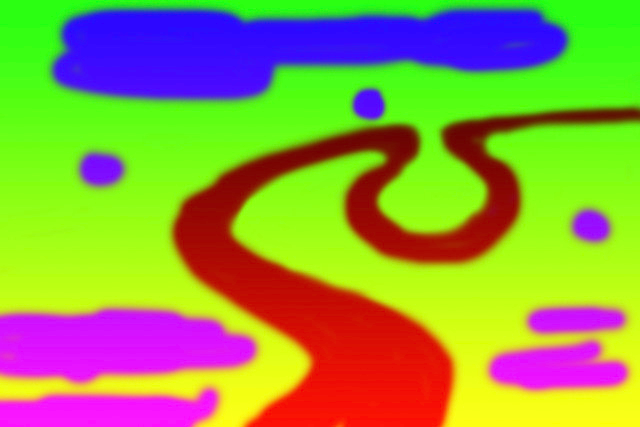
\includegraphics[height=55pt]{files/assets/articles/hz3.png}}
	& $:$ &
	\raisebox{-.5\height}{
	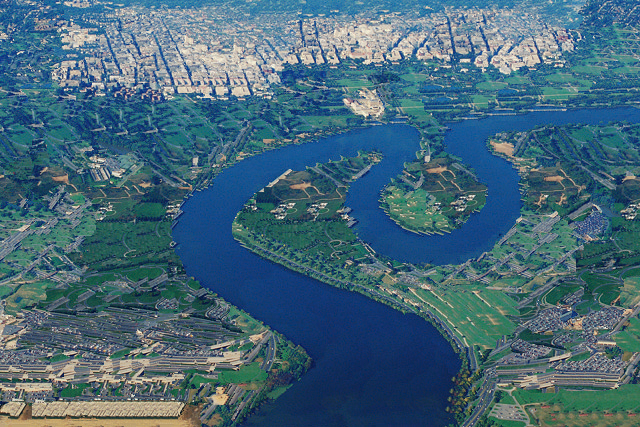
\includegraphics[height=55pt]{files/assets/articles/hz4.png}}\\
	$A$&&$A'$&&$B$&&$B'$
	\end{tabular}

	\caption{Outro exemplo de analogia de textura. Este
	exemplo mostra que o método também pode receber 
	um descritor de uma imagem para gerar outra.}
	\label{img:preview}
\end{figure}

\newpage
\section{Transferência de estilo} 

O método de ``Style Transfer'' proposto
por Gatys, Ecker e Bethge \cite{Gatys2016}
permite, alem de re-amostrar a textura,
controlar a geometria do resultado.
Para isso o algoritmo recebe duas imagens,
uma definirá o estilo
e outra definirá o conteúdo do resultado.
Apesar de produzir resultados bem interessantes,
tendo implementado o método de síntese de
textura, a transferência de estilo
só exige um pequeno passo a mais.


Para implementar o método, é preciso
gerar as representações da imagem de
conteúdo na rede convolucional.
Então, basta adicionar
à função de perda a diferença entre
a representação da imagem gerada e do
conteúdo. Assim vão existir duas perdas,
$\mathcal{L}_{content}$ que representa
a perda do conteúdo com as representações
da rede, e $\mathcal{L}_{style}$, que
representa a perda com as matrizes de Gram.
%CITAR IMAGEM




\begin{figure}[!ht]
	\centering
	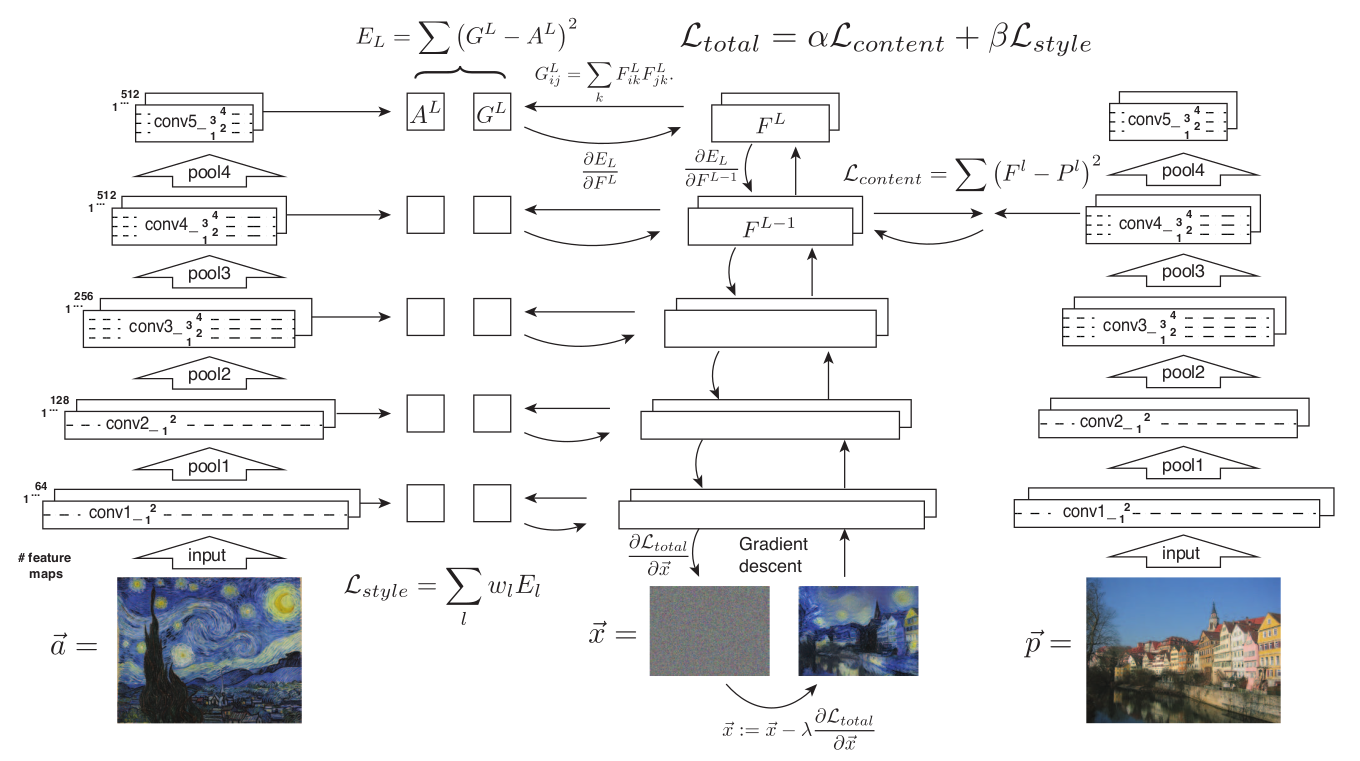
\includegraphics[width=\linewidth]{files/assets/articles/gatys3.png}
	\caption{Método da transferência de estilo. Faz a otimização
	das matrizes de Gram e das Features ao mesmo tempo.}
	\label{img:preview}
\end{figure}


% Definir e mostrar resultados

% Falar do deepart.io?

\fi